\documentclass[border=8pt]{standalone}
\usepackage{tikz}
\usetikzlibrary{arrows.meta,positioning,calc}
\begin{document}
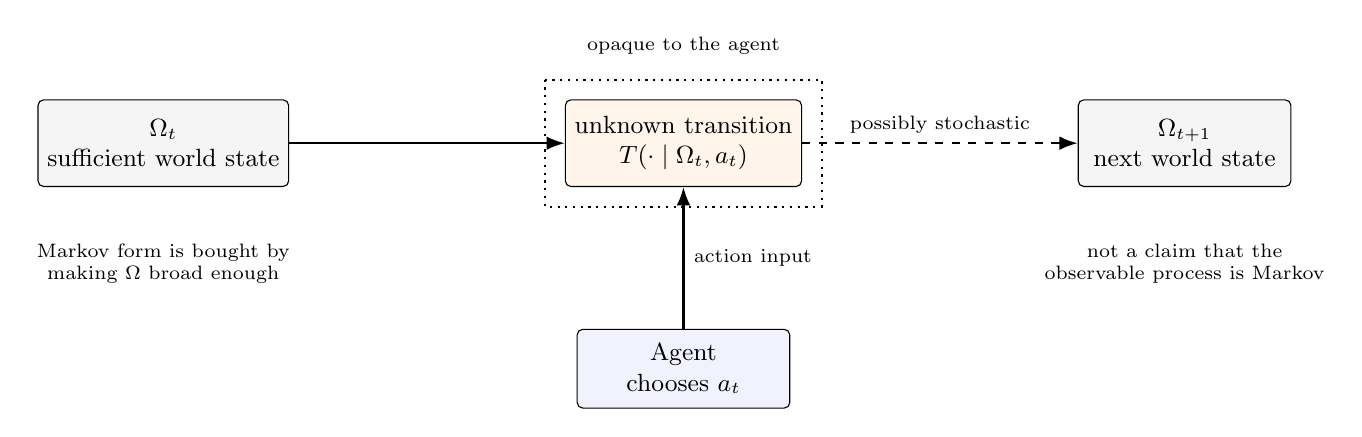
\begin{tikzpicture}[
  state/.style={draw, rounded corners=2pt, align=center, minimum width=2.7cm, minimum height=1.1cm, font=\small},
  kernel/.style={draw, rounded corners=2pt, align=center, minimum width=3.0cm, minimum height=1.1cm, font=\small, fill=orange!8},
  agent/.style={draw, rounded corners=2pt, align=center, minimum width=2.7cm, minimum height=1.0cm, font=\small, fill=blue!5},
  arr/.style={-Latex, thick},
  hidden/.style={-Latex, thick, dashed},
  note/.style={align=center, font=\scriptsize}
]

\node[state, fill=gray!8] (omega0) {$\Omega_t$\\sufficient world state};
\node[kernel, right=3.5cm of omega0] (T) {unknown transition\\$T(\cdot\mid\Omega_t,a_t)$};
\node[state, fill=gray!8, right=3.5cm of T] (omega1) {$\Omega_{t+1}$\\next world state};
\node[agent, below=1.8cm of T] (agent) {Agent\\chooses $a_t$};

\draw[arr] (omega0) -- (T);
\draw[hidden] (T) -- node[above, note] {possibly stochastic} (omega1);
\draw[arr] (agent) -- node[right, note] {action input} (T);

\draw[thick, dotted] ($(T.north west)+(-0.25,0.25)$) rectangle ($(T.south east)+(0.25,-0.25)$);
\node[note, above=0.45cm of T] {opaque to the agent};

\node[note, below=0.6cm of omega0] {Markov form is bought by\\making $\Omega$ broad enough};
\node[note, below=0.6cm of omega1] {not a claim that the\\observable process is Markov};

\end{tikzpicture}
\end{document}
